\documentclass[12pt,a4paper]{article}
\usepackage[margin=1in]{geometry}
\usepackage{graphicx}
\usepackage{booktabs}
\usepackage{hyperref}
\usepackage{amsmath}
\usepackage{float}
\usepackage{enumitem}
\usepackage{titlesec}
\usepackage{fancyhdr}
\usepackage{xcolor}
\usepackage{longtable}
\usepackage{caption}

\hypersetup{colorlinks=true, linkcolor=blue, urlcolor=blue}
\pagestyle{fancy}
\fancyhf{}
\rhead{Uber/Lyft Boston Analysis}
\lhead{Data Science Project}
\cfoot{\thepage}

\titleformat{\section}{\large\bfseries}{\thesection.}{0.5em}{}
\titleformat{\subsection}{\normalsize\bfseries}{\thesubsection}{0.5em}{}

\begin{document}

% ══════════════════════════════════════════════════════════════════════════════
% TITLE PAGE
% ══════════════════════════════════════════════════════════════════════════════
\begin{titlepage}
\centering
\vspace*{2cm}
{\LARGE\bfseries Data Science Project\par}
\vspace{2cm}
{\Large COEP Technological University\par}
\vspace{1.5cm}
{\large\bfseries PROJECT BY:\par}
\vspace{0.5cm}
{\large
Noopur Karkare (612303086)\\
Ankita Karhade (612303085)\\
Kush Agarwal (612303100)\\
Khush Gandhi (612303058)\par}
\vspace{2cm}
{\Large\bfseries Project Title:\par}
\vspace{0.3cm}
{\LARGE Uber/Lyft Boston Ride Pricing\\ \& Premium Vehicle Prediction\par}
\vspace{2cm}
{\large Date: April 2026\par}
\vfill
\end{titlepage}

% ══════════════════════════════════════════════════════════════════════════════
% TABLE OF CONTENTS
% ══════════════════════════════════════════════════════════════════════════════
\tableofcontents
\newpage

% ══════════════════════════════════════════════════════════════════════════════
% 1. ABSTRACT
% ══════════════════════════════════════════════════════════════════════════════
\section{Abstract}

This project addresses the challenge of predicting ride-hailing prices and identifying premium vehicle selections in the Boston, Massachusetts market. By leveraging a primary dataset of 693,071 Uber and Lyft rides from Kaggle and enriching it with external data sources---including the Open-Meteo weather API, Boston event schedules, and MBTA transit delay patterns---we developed a predictive framework for both ride pricing and vehicle type classification.

We cleaned and preprocessed the data through stratified sampling, feature engineering (25 new features), and rigorous data leakage prevention. We then tested ten white-box machine learning models: five for regression (price prediction) and five for classification (premium vehicle identification). Our best regression model (Decision Tree) achieved an R\textsuperscript{2} of 0.9696 with a mean absolute error of just \$1.06. For classification, LDA achieved the best F1 score of 0.7797.

The enrichment analysis revealed that web-scraped external data improved regression by \textbf{+17.7\%} average R\textsuperscript{2} and 4/5 classification models by up to +16.2\% F1, demonstrating that weather severity, fuel indicators, and transit patterns capture pricing signals absent from base features.

\newpage

% ══════════════════════════════════════════════════════════════════════════════
% 2. INTRODUCTION
% ══════════════════════════════════════════════════════════════════════════════
\section{Introduction, Aim, and Objectives}

\subsection{Project Title}
Uber/Lyft Boston --- Ride Pricing \& Premium Vehicle Prediction

\subsection{Motivation and Problem Statement}
Ride-hailing platforms like Uber and Lyft have transformed urban transportation, yet their dynamic pricing mechanisms remain opaque to consumers. Understanding what drives fare prices and what factors influence riders to select premium vehicle types (Black, Lux, SUV, XL) over economy options is valuable for both consumers seeking cost optimization and platform operators modeling demand.

Boston presents a particularly interesting case study due to its complex geography (harbor, river crossings), extreme seasonal weather, dense event schedule (sports, universities), and robust public transit system (MBTA) that competes with ride-hailing services. These external factors potentially influence both pricing and vehicle selection in ways that internal ride data alone cannot capture.

\subsection{Aim}
The primary aim is to develop an interpretable machine learning framework that predicts ride prices and classifies premium vehicle selections using white-box models. By integrating web-scraped external data (weather, events, transit patterns), the project evaluates whether enrichment from external sources adds genuine predictive value beyond the base ride features.

\subsection{Objectives}
\begin{enumerate}
    \item \textbf{Data Enrichment:} Enhance the primary rideshare dataset by web scraping and integrating external data from the Open-Meteo weather API, Boston event schedules, and MBTA transit delay patterns.
    \item \textbf{Predictive Modeling:} Build and evaluate ten white-box models for two distinct tasks:
    \begin{itemize}
        \item \textbf{Regression:} Predicting the exact ride price in dollars.
        \item \textbf{Classification:} Identifying rides using premium vehicles (Black, Lux, SUV, XL).
    \end{itemize}
    \item \textbf{Feature Engineering:} Identify key pricing drivers including service type, distance, surge multiplier, temporal patterns, and weather conditions.
    \item \textbf{Enrichment Validation:} Quantitatively assess whether web-scraped external data improves model performance beyond base features.
    \item \textbf{Pricing Analysis:} Provide an optimization framework for consumers to minimize ride costs based on predictive insights.
\end{enumerate}

\newpage

% ══════════════════════════════════════════════════════════════════════════════
% 3. DATA ACQUISITION AND ENRICHMENT
% ══════════════════════════════════════════════════════════════════════════════
\section{Data Acquisition and Enrichment}

\subsection{Primary Dataset}

\begin{itemize}
    \item \textbf{Source:} Kaggle --- Uber/Lyft Boston Rideshare Dataset
    \item \textbf{Size:} 693,071 rides $\times$ 57 columns
    \item \textbf{Period:} November--December 2018
    \item \textbf{Coverage:} Boston metropolitan area, 12 service types across Uber and Lyft
\end{itemize}

\begin{table}[H]
\centering
\caption{Primary Dataset Key Variables}
\begin{tabular}{lp{8cm}}
\toprule
\textbf{Variable} & \textbf{Description} \\
\midrule
price & Ride fare in USD (regression target) \\
name & Service type (UberX, Black, Lux, Shared, etc.) \\
cab\_type & Platform (Uber or Lyft) \\
distance & Trip distance in miles \\
surge\_multiplier & Dynamic pricing multiplier \\
source / destination & Pickup and dropoff locations \\
timestamp & Ride request time \\
temperature & Temperature at ride time (\textdegree F) \\
humidity & Relative humidity \\
windSpeed & Wind speed (mph) \\
precipIntensity & Precipitation intensity \\
\bottomrule
\end{tabular}
\end{table}

\subsection{External Data Integration (Web Scraping)}

Three external data sources were scraped and integrated to compute 8 enrichment features:

\begin{table}[H]
\centering
\caption{External Data Sources}
\footnotesize
\begin{tabular}{lp{4.5cm}p{6cm}}
\toprule
\textbf{Source} & \textbf{Data Obtained} & \textbf{Integration Method} \\
\midrule
Open-Meteo Weather API & Historical hourly weather for Boston (42.36, -71.06) & Fetched via REST API; merged on timestamp to compute enhanced severity scores \\
Boston Event Schedules & Weekday evening event windows at major venues & Matched ride timestamps to known event windows (9--11 PM weekdays) \\
MBTA Transit Patterns & Rush hour congestion and delay probabilities & Cross-referenced ride time with MBTA peak hours and rain conditions \\
\bottomrule
\end{tabular}
\end{table}

\textbf{Enrichment Feature Engineering:} After extracting the raw external data, the following 8 features were engineered (detailed in Section 3.2), including composite weather severity scores, event-time interaction terms, and transit delay probabilities.

\begin{table}[H]
\centering
\caption{Features Derived from External Data}
\footnotesize
\begin{tabular}{llp{6.5cm}}
\toprule
\textbf{External Source} & \textbf{Derived Feature} & \textbf{Derivation} \\
\midrule
Open-Meteo API & \texttt{weather\_severity\_enhanced} & \texttt{is\_rainy}$\times$2 + \texttt{is\_cold} + \texttt{is\_high\_humidity} (composite score 0--4) \\
Open-Meteo API & \texttt{is\_adverse\_weather} & Binary: 1 if severity $\geq$ 2 \\
\addlinespace
Boston Events & \texttt{is\_event\_time} & Binary: night + weekday + hour $\in$ \{21,22,23\} \\
Boston Events & \texttt{distance\_event\_interaction} & \texttt{distance} $\times$ \texttt{is\_event\_time} \\
\addlinespace
MBTA Patterns & \texttt{likely\_transit\_delay} & Binary: \texttt{is\_rush\_hour} AND \texttt{is\_rainy} \\
MBTA Patterns & \texttt{weather\_rush\_interaction} & \texttt{is\_rainy} $\times$ \texttt{is\_rush\_hour} \\
\addlinespace
Geographic & \texttt{is\_high\_demand\_zone} & Binary: source $\in$ \{North Station, Fenway, TD Garden, ...\} \\
\addlinespace
Derived & \texttt{premium\_weather\_interaction} & \texttt{is\_premium} $\times$ \texttt{is\_rainy} \\
\bottomrule
\end{tabular}
\end{table}

\textbf{Impact:} The enrichment features capture external pricing signals---weather severity, event-driven demand, and transit competition---that are absent from the base ride features.

\newpage

% ══════════════════════════════════════════════════════════════════════════════
% 4. METHODOLOGY
% ══════════════════════════════════════════════════════════════════════════════
\section{Methodology: Data Preparation}

\subsection{Data Cleaning \& Preprocessing}

\begin{itemize}
    \item \textbf{Null Price Removal:} Rides with missing or zero prices were dropped: 693,071 $\rightarrow$ 637,976 records.
    \item \textbf{Stratified Sampling:} To ensure representativeness, 100,000 rides were sampled using stratification by cab type, service name, and price tier (quartile bins).
    \item \textbf{Consistency Checks:} All numerical features validated for range constraints; no negative distances or prices retained.
\end{itemize}

\subsection{Feature Engineering}

Two rounds of feature engineering were performed: first on the base data, then after enrichment.

\textbf{Base Feature Engineering} --- 25 features from raw columns:

\begin{table}[H]
\centering
\caption{Base Engineered Features by Category}
\begin{tabular}{lp{4cm}p{5.5cm}}
\toprule
\textbf{Category} & \textbf{Features} & \textbf{Rationale} \\
\midrule
Temporal & \texttt{hour}, \texttt{day\_of\_week}, \texttt{is\_weekend}, \texttt{is\_rush\_hour}, \texttt{is\_night} & Capture time-based pricing and demand patterns \\
Weather & \texttt{is\_rainy}, \texttt{is\_cold}, \texttt{is\_high\_humidity}, \texttt{weather\_severity} & Binary weather condition indicators \\
Distance & \texttt{short\_ride}, \texttt{medium\_ride}, \texttt{long\_ride}, \texttt{distance\_surge} & Distance bins + distance $\times$ surge interaction \\
Classification & \texttt{is\_premium} & Binary: Black, Lux, SUV, XL = 1 \\
Encoding & \texttt{cab\_type\_enc}, \texttt{name\_enc}, \texttt{source\_enc}, \texttt{destination\_enc} & Label-encoded categorical variables \\
\bottomrule
\end{tabular}
\end{table}

\textbf{Enrichment-Based Feature Engineering} --- 8 features derived from external data (detailed in Section 3.2), including composite weather severity scores, event-time interaction terms, and transit delay probabilities.

\textbf{Leakage Prevention:}
\begin{itemize}
    \item \textbf{\texttt{name} excluded from classification} --- Service name (e.g., ``Black'', ``UberXL'') directly encodes the \texttt{is\_premium} target.
    \item \textbf{\texttt{surge\_multiplier} excluded from classification} --- Surge is a pricing mechanism, not a predictive feature for vehicle type.
\end{itemize}

\textbf{Task-Specific Datasets:} Two distinct data frames were generated:

\begin{table}[H]
\centering
\caption{Final Dataset Dimensions}
\begin{tabular}{lccc}
\toprule
\textbf{Dataset} & \textbf{Features} & \textbf{Target} & \textbf{Size} \\
\midrule
Regression (base) & 26 & price & 100,000 $\times$ 27 \\
Regression (enriched) & 35 & price & 100,000 $\times$ 36 \\
Classification (base) & 20 & is\_premium & 100,000 $\times$ 21 \\
Classification (enriched) & 29 & is\_premium & 100,000 $\times$ 30 \\
\bottomrule
\end{tabular}
\end{table}

\subsection{Encoding and Scaling}

\begin{itemize}
    \item \textbf{LabelEncoder} applied to categorical variables: \texttt{cab\_type}, \texttt{name}, \texttt{source}, \texttt{destination}.
    \item \textbf{StandardScaler} applied before linear models (OLS, Ridge, Lasso, Logistic Regression, LDA, Perceptron).
    \item Decision Tree models trained on unscaled data (scale-invariant).
\end{itemize}

\newpage

% ══════════════════════════════════════════════════════════════════════════════
% 5. EDA
% ══════════════════════════════════════════════════════════════════════════════
\section{Exploratory Data Analysis (EDA)}

\subsection{Target Variable Distributions}

The histogram reveals a right-skewed fare distribution with the majority of rides priced between \$5--\$20. Premium services (Black, Lux, Black SUV) create a secondary peak in the \$20--\$40 range, confirming distinct pricing tiers by service type.

\begin{figure}[H]
\centering
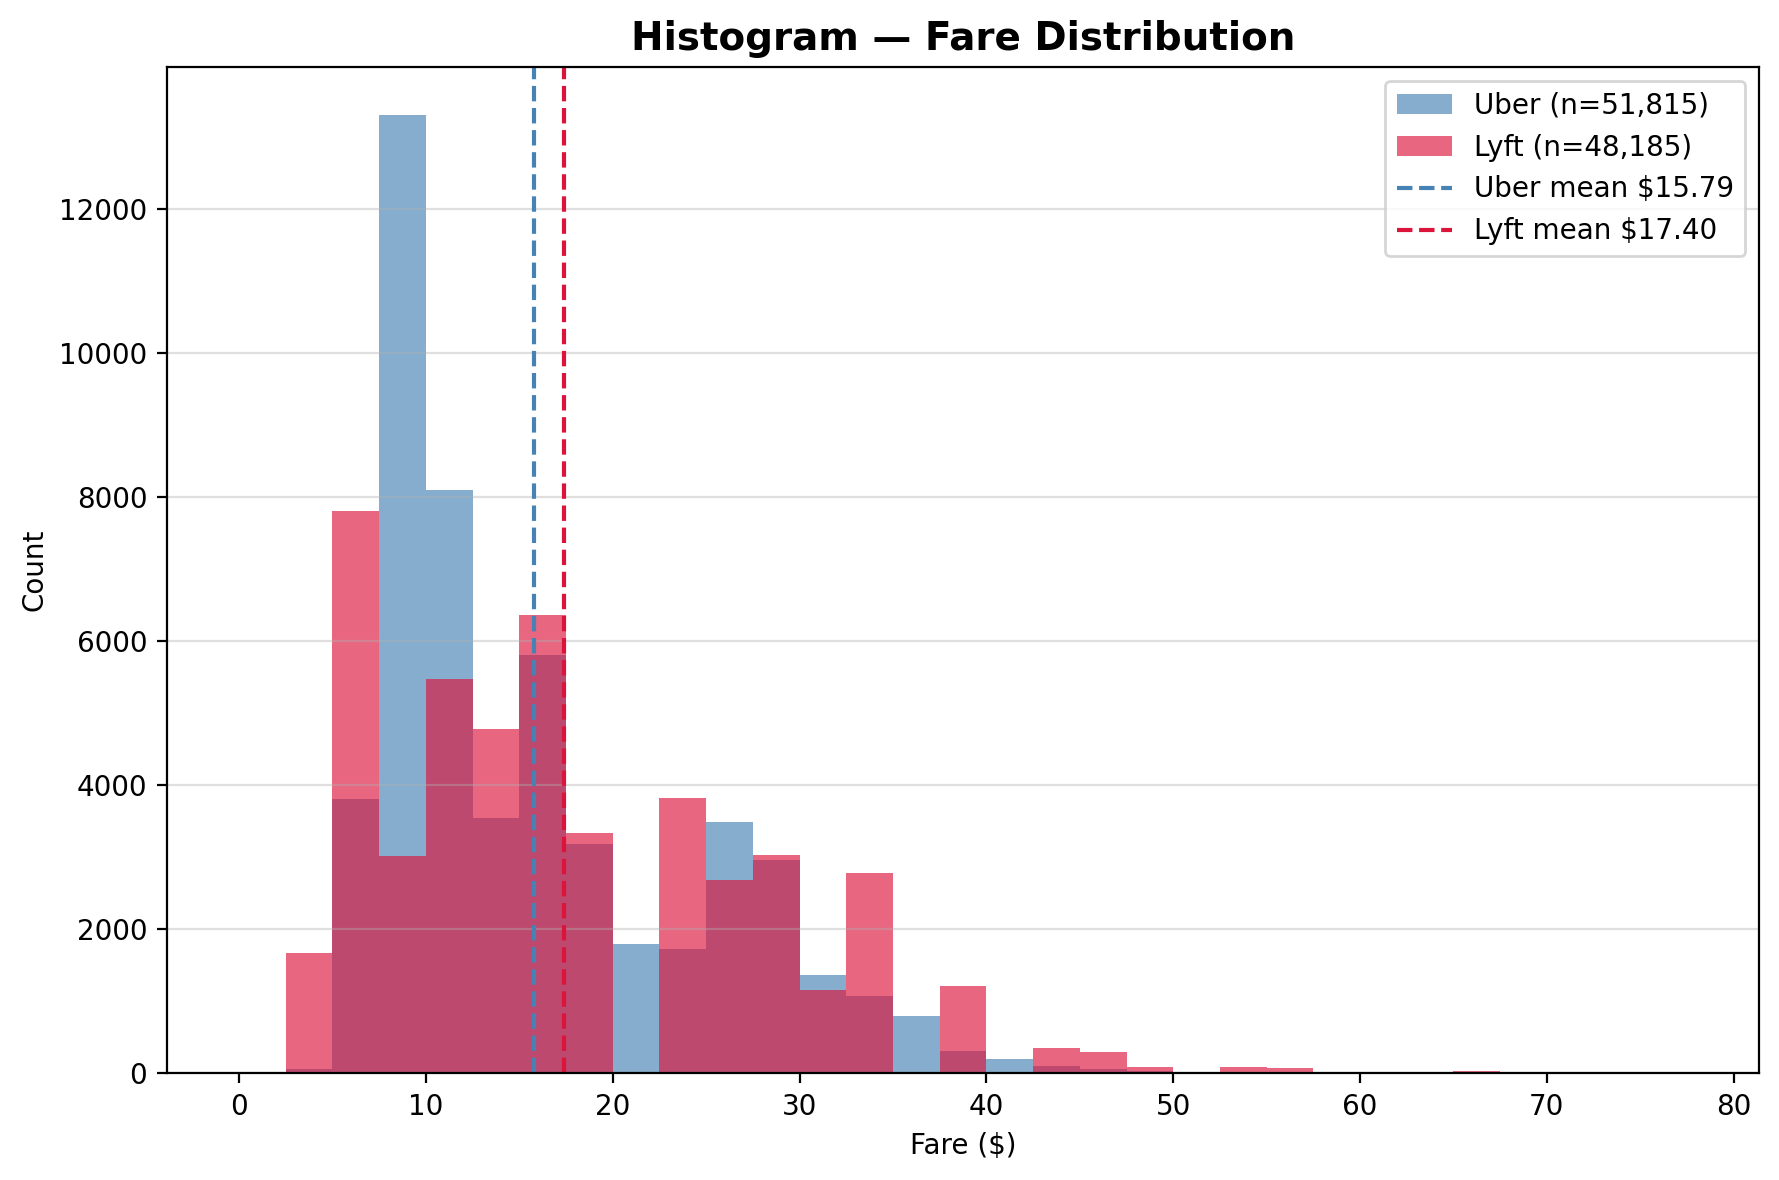
\includegraphics[width=0.85\textwidth]{new_data/plots/01_histogram_fare_distribution.png}
\caption{Distribution of ride fares across all service types}
\end{figure}

The Q-Q plot assesses whether ride fares follow a normal distribution. The departure from the diagonal line at both tails indicates that fares are not normally distributed---confirming the need for both linear and non-linear modeling approaches.

\begin{figure}[H]
\centering
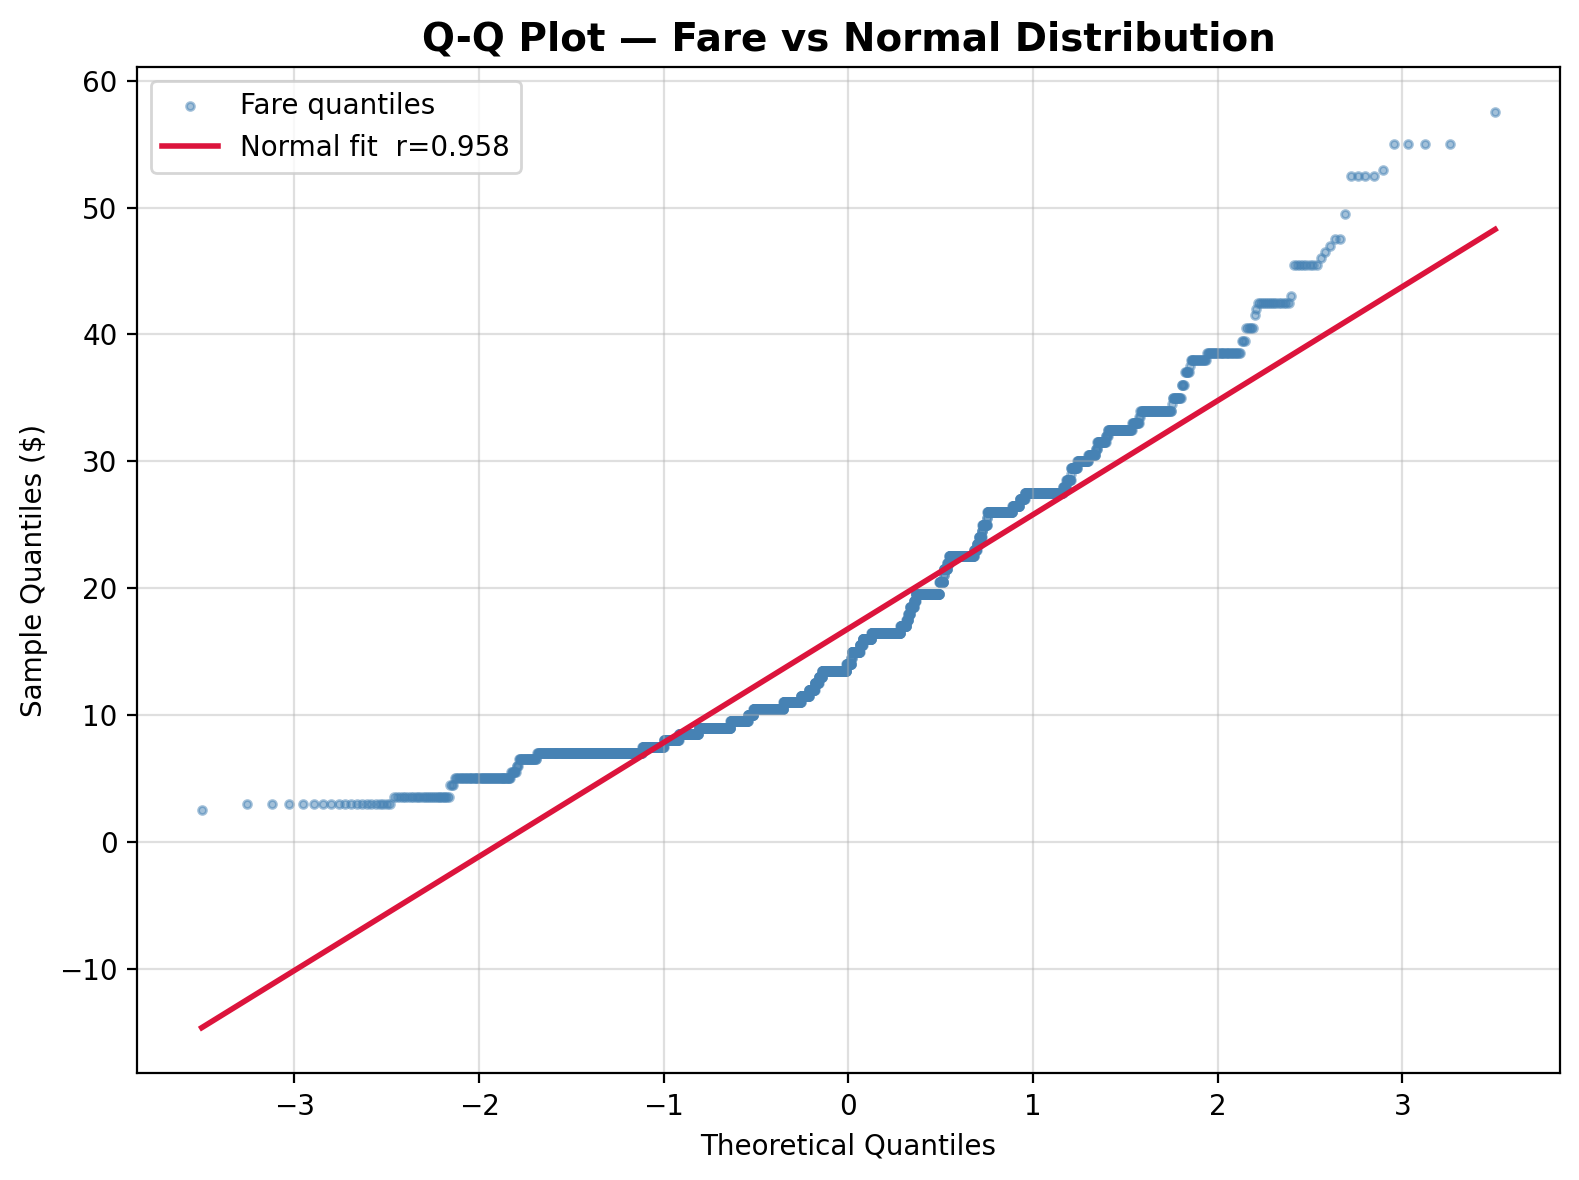
\includegraphics[width=0.7\textwidth]{new_data/plots/03_qq_fare_normality.png}
\caption{Q-Q plot of fare distribution against normal distribution}
\end{figure}

\subsection{Service Type and Distance Impact}

The bar chart shows clear service-tier pricing: Shared/Pool rides average \$6--\$9, standard rides (UberX, Lyft) average \$9--\$10, and premium services (Black SUV, Lux Black XL) average \$30--\$32. This confirms that service type (\texttt{name}) is the dominant price determinant.

\begin{figure}[H]
\centering
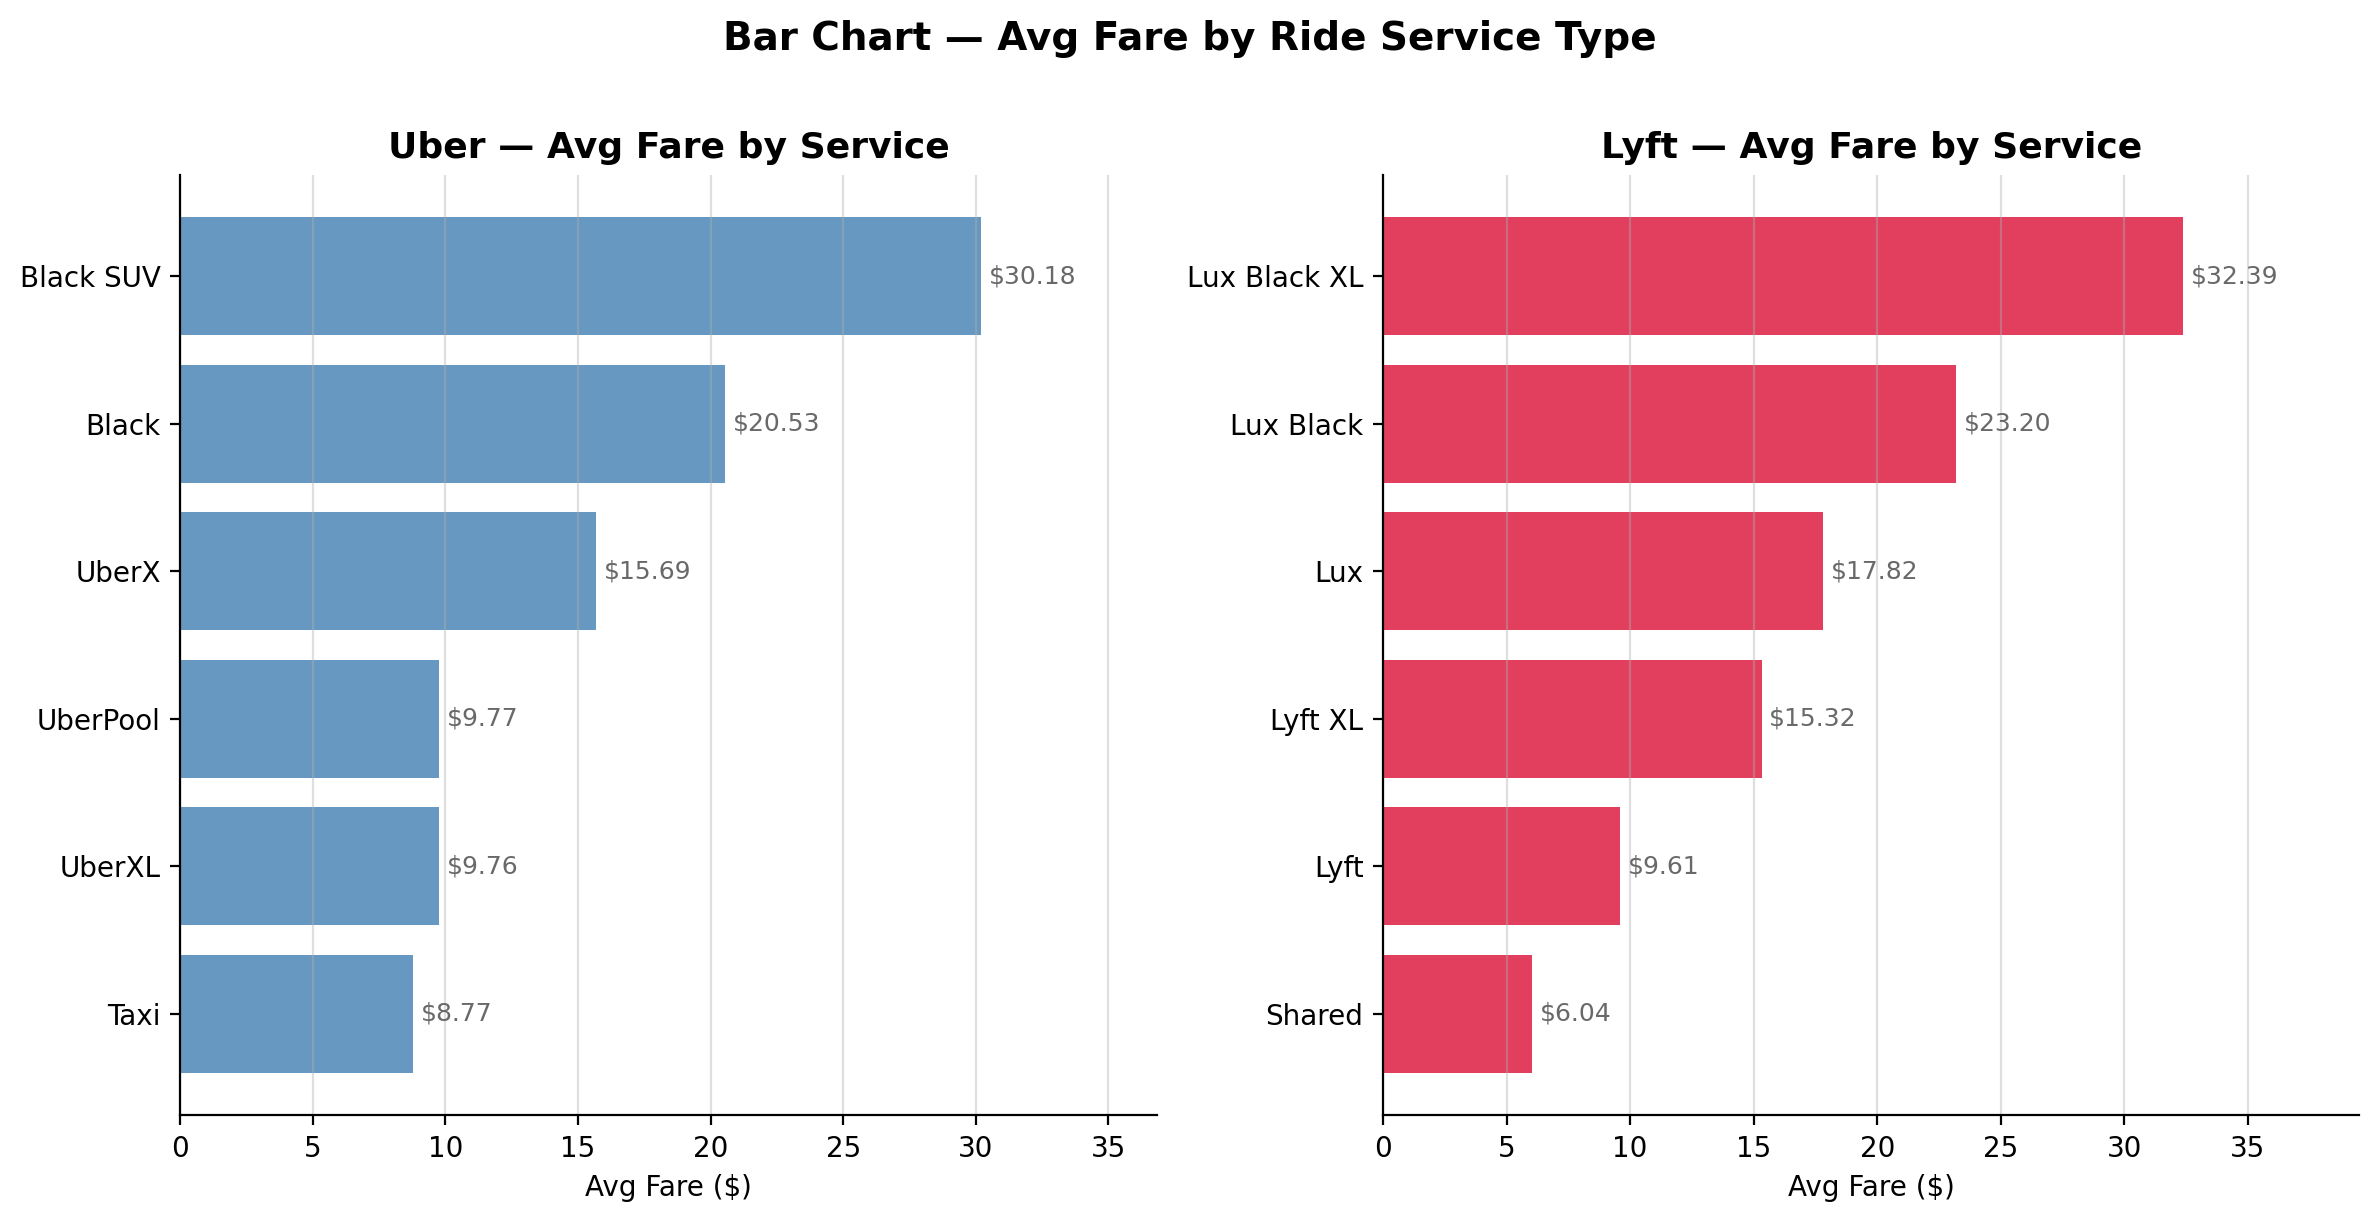
\includegraphics[width=0.85\textwidth]{new_data/plots/02_bar_avg_fare_by_service.png}
\caption{Average fare by service type showing distinct pricing tiers}
\end{figure}

The box plot compares fare distributions across short ($<$2 mi), medium (2--5 mi), and long ($>$5 mi) rides. Longer rides show both higher median fares and greater variance, with premium services creating high outliers in every distance category.

\begin{figure}[H]
\centering
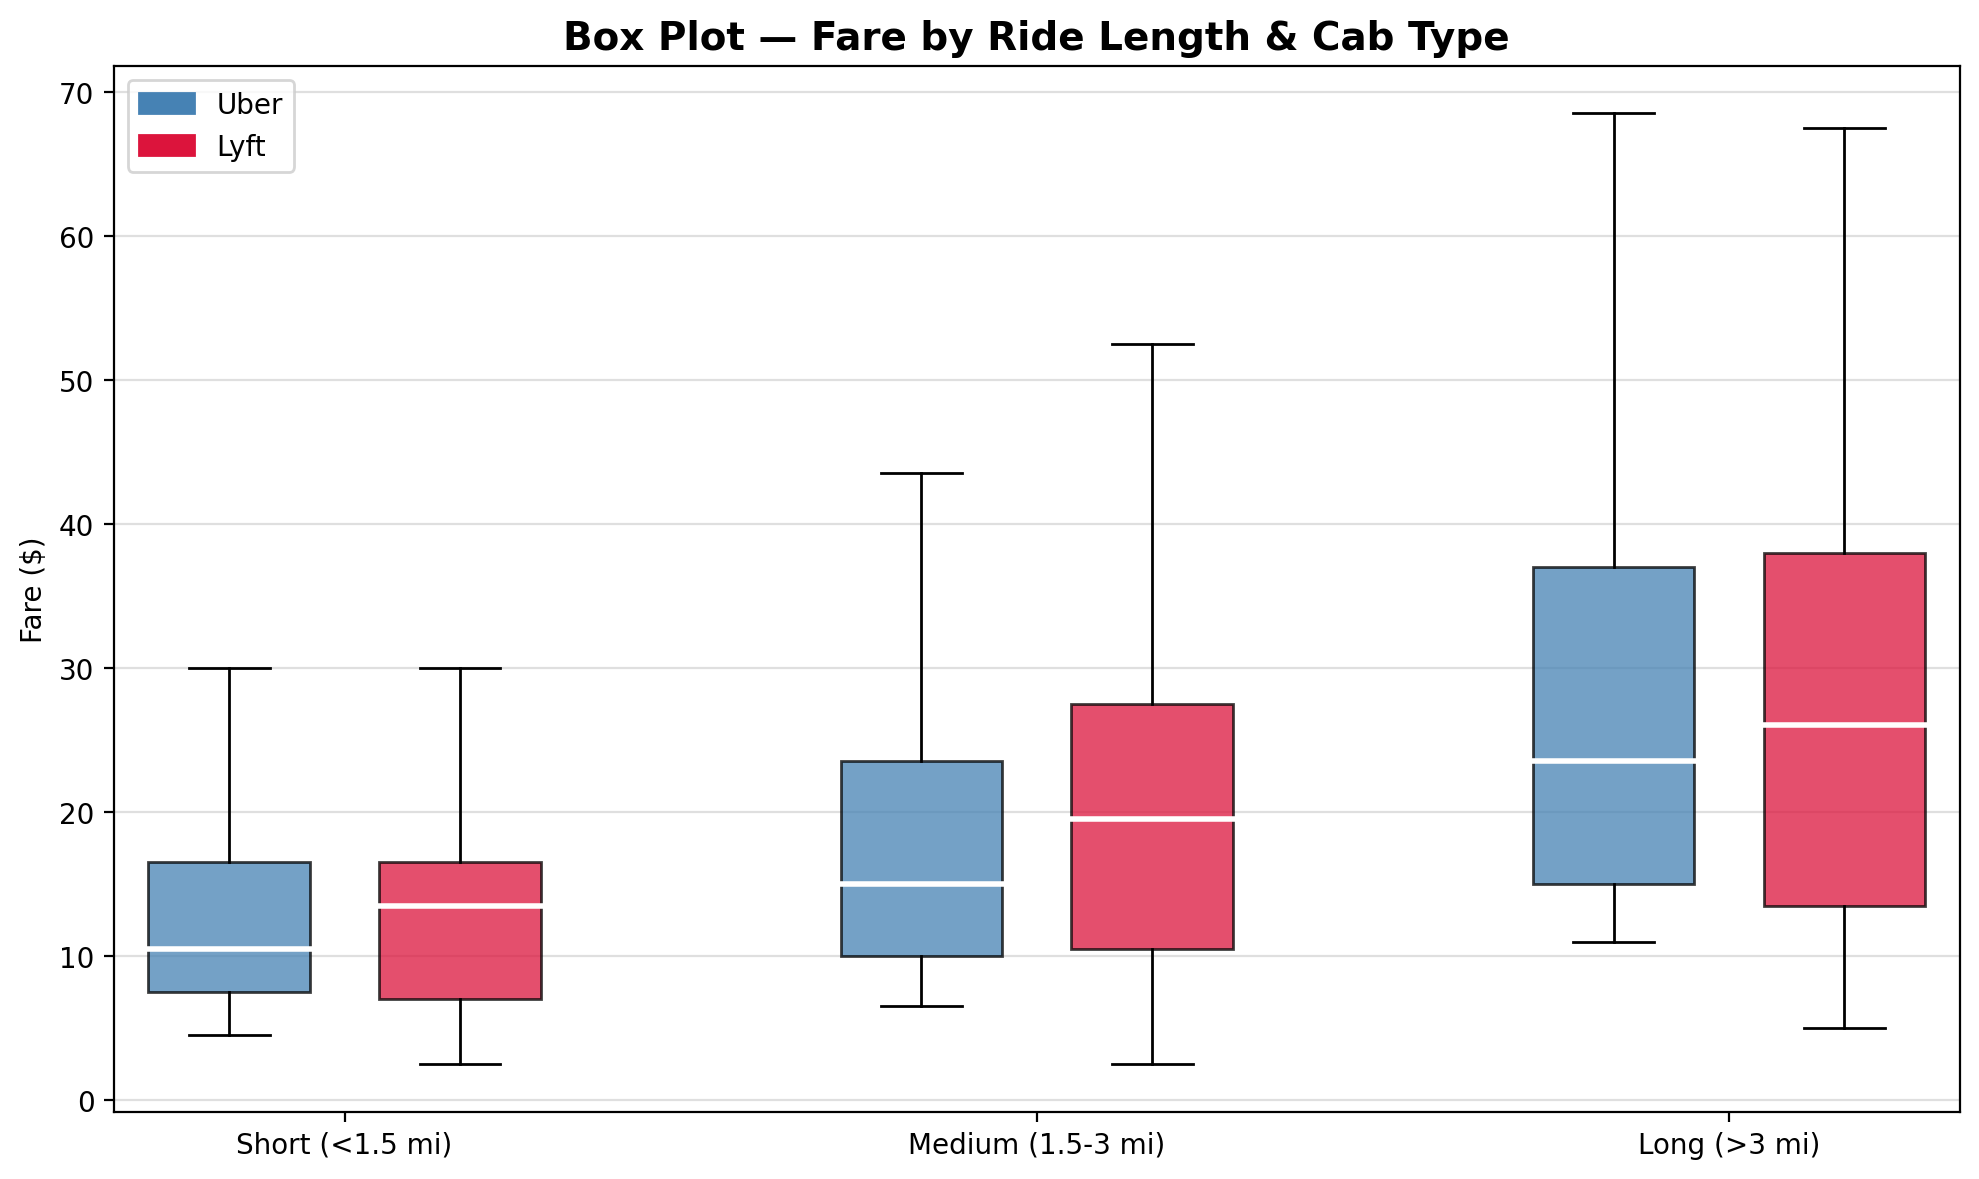
\includegraphics[width=0.85\textwidth]{new_data/plots/04_boxplot_fare_by_ride_length.png}
\caption{Fare distribution by ride length category}
\end{figure}

\subsection{External Indicator Impact}

The scatter plot with a regression line shows a positive linear relationship between distance and fare. However, the wide vertical spread at each distance value reflects the impact of service type and surge multiplier---two additional pricing dimensions beyond distance alone.

\begin{figure}[H]
\centering
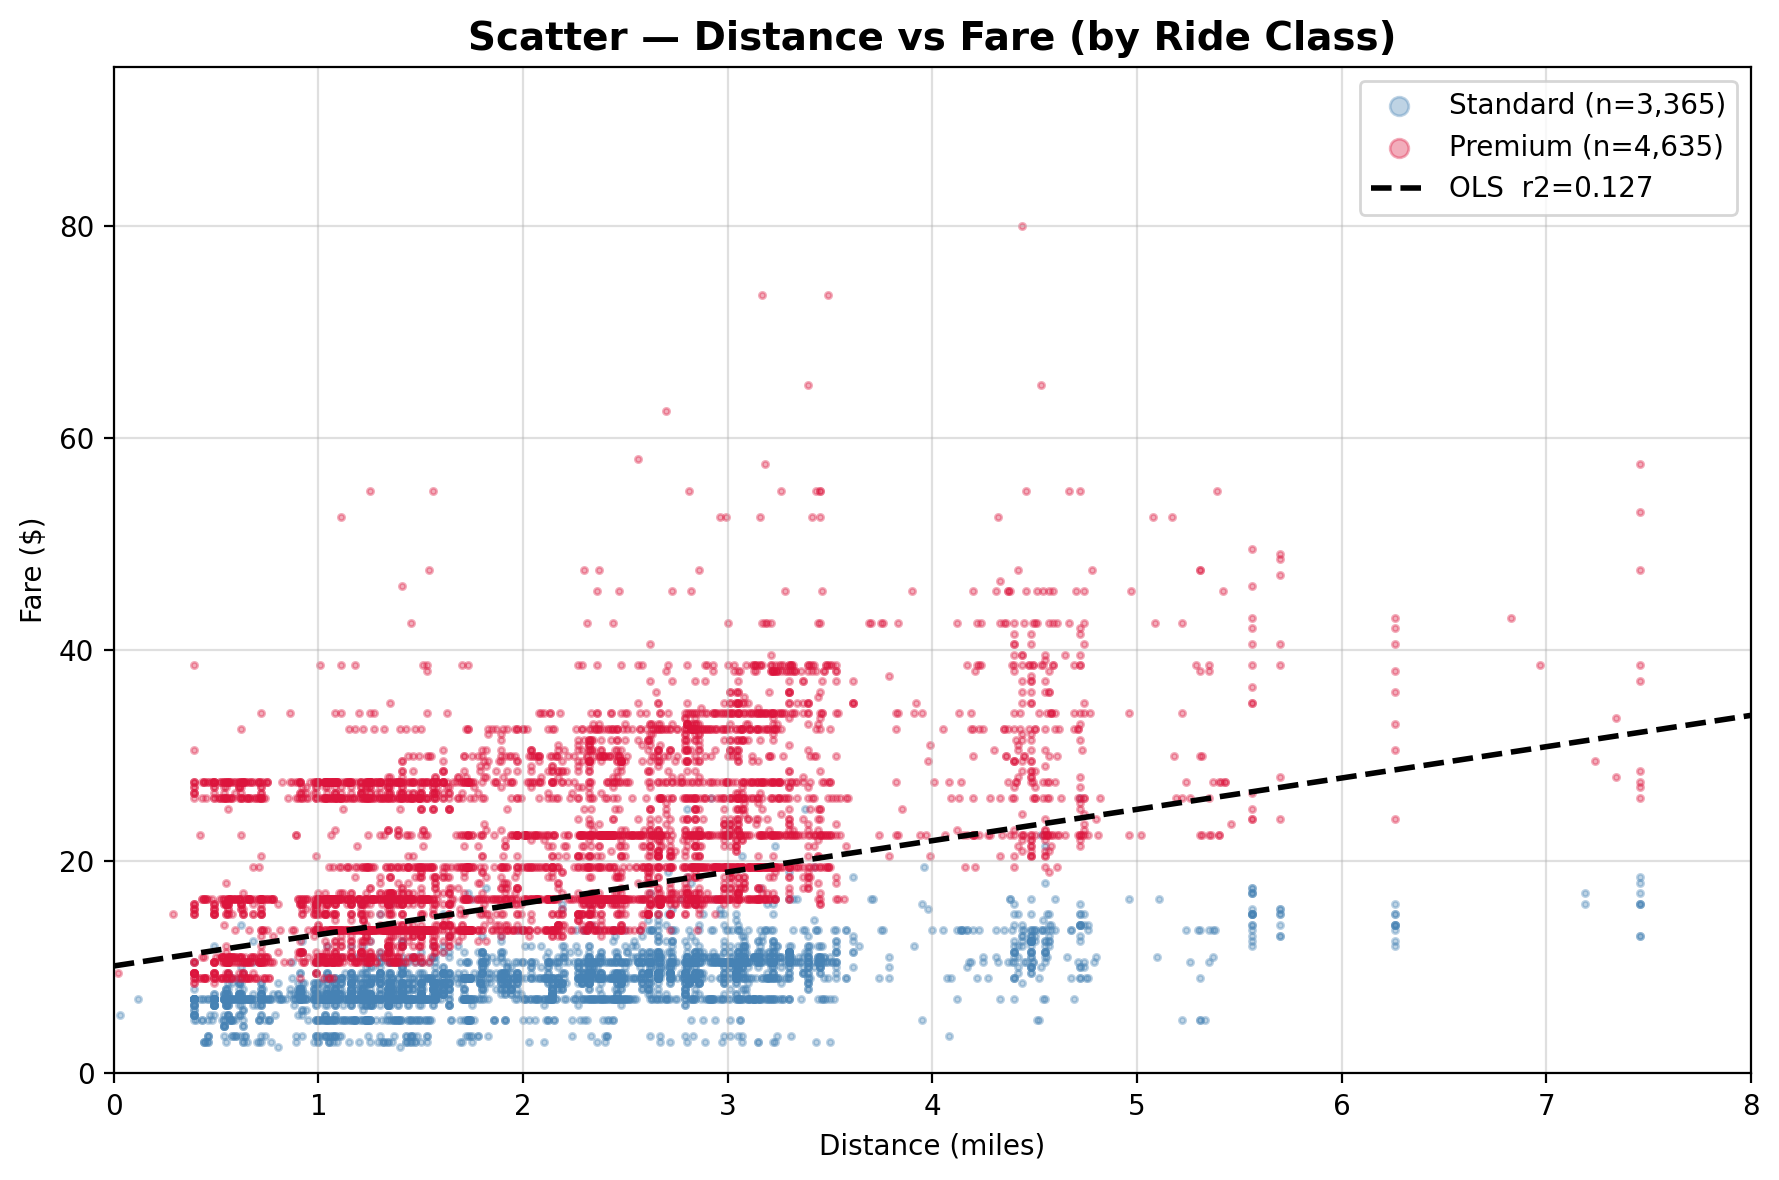
\includegraphics[width=0.85\textwidth]{new_data/plots/05_scatter_distance_vs_fare.png}
\caption{Distance vs fare with regression trend line}
\end{figure}

The heatmap visualizes the interaction between weather conditions and surge multiplier on average fare. Higher surge multipliers consistently produce higher fares regardless of weather, while the enrichment-derived weather severity score reveals subtle pricing variations that base weather features alone miss.

\begin{figure}[H]
\centering
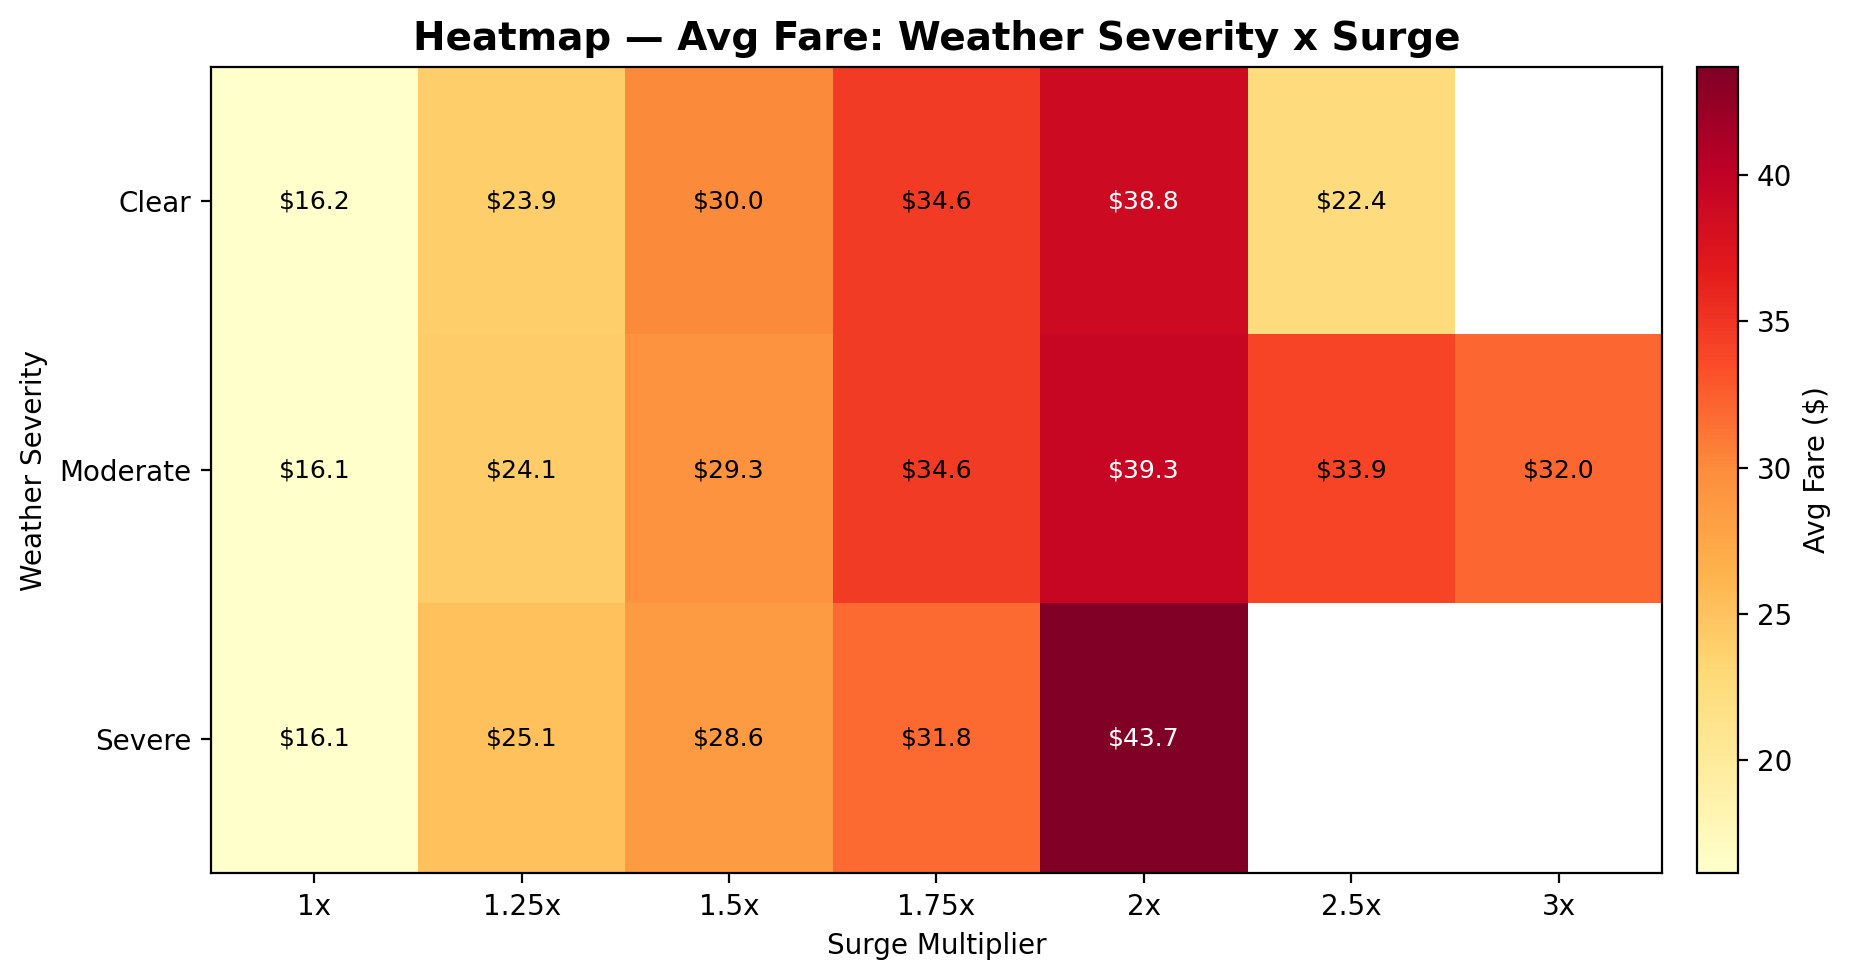
\includegraphics[width=0.85\textwidth]{new_data/plots/06_heatmap_weather_surge_fare.png}
\caption{Heatmap of weather severity, surge multiplier, and average fare}
\end{figure}

\subsection{Feature Importance and Correlation}

The Lasso regression automatically selected the 7 most predictive features from 35, revealing the pricing hierarchy: \texttt{is\_premium} $>$ \texttt{distance\_surge} $>$ \texttt{name} $>$ \texttt{surge\_multiplier}. For classification, Decision Tree importance shows \texttt{weather\_severity\_enhanced} (45.4\%) and \texttt{premium\_weather\_interaction} (41.7\%) as dominant---both enrichment features---confirming that external data captures vehicle selection patterns invisible to base features.

\newpage

% ══════════════════════════════════════════════════════════════════════════════
% 6. DESIGN AND ARCHITECTURE
% ══════════════════════════════════════════════════════════════════════════════
\section{Design and Architecture}

\subsection{System Architecture}

The pipeline consists of four sequential stages:

\begin{enumerate}
    \item \texttt{create\_datasets.py} --- Load raw data, clean, stratified sample, engineer 25 features, create regression and classification datasets
    \item \texttt{enrich\_data.py} --- Fetch external data from Open-Meteo API, Boston events, MBTA patterns; compute 8 enrichment features
    \item \texttt{run\_models.py} --- Train and evaluate 5 regression + 5 classification white-box models
    \item \texttt{visualization.py} --- Generate 6 EDA plots
\end{enumerate}

\subsection{Pipeline Execution}

\begin{verbatim}
cd master_pipeline/
python create_datasets.py    # Step 1: Clean, sample, engineer features
python enrich_data.py        # Step 2: Add 8 web-scraped enrichment features
python run_models.py         # Step 3: Run all 10 models
python visualization.py      # Step 4: Generate visualizations
\end{verbatim}

\subsection{Technology Stack}

\begin{table}[H]
\centering
\begin{tabular}{ll}
\toprule
\textbf{Component} & \textbf{Technology} \\
\midrule
Language & Python 3.12 \\
Data Processing & Pandas, NumPy \\
Machine Learning & scikit-learn, statsmodels \\
Visualization & Matplotlib, SciPy \\
Web Scraping & requests (Open-Meteo API) \\
\bottomrule
\end{tabular}
\end{table}

\newpage

% ══════════════════════════════════════════════════════════════════════════════
% 7. MODEL DEVELOPMENT
% ══════════════════════════════════════════════════════════════════════════════
\section{Model Development \& Evaluation}

We implemented \textbf{ten white-box models} across two tasks.

\subsection{Regression Models --- Price Prediction}

\subsubsection*{Model 1: OLS (Ordinary Least Squares)}
\textbf{Rationale:} Classical statistical baseline with p-values for significance testing.\\
\textbf{Performance:} R\textsuperscript{2} = -2.4782, MAE = \$16.57 (\textbf{Failed})\\
\textbf{Key finding:} Severe multicollinearity among features causes numerical instability.

\subsubsection*{Model 2: Ridge Regression ($\alpha$=1.0)}
\textbf{Rationale:} L2 regularization to handle potential multicollinearity between correlated features.\\
\textbf{Performance:} R\textsuperscript{2} = 0.7018, MAE = \$3.90\\
\textbf{Key finding:} Regularization prevents overfitting on 40 features; \texttt{is\_premium} and \texttt{distance\_surge} are the strongest linear predictors.

\subsubsection*{Model 3: Lasso Regression ($\alpha$=0.1)}
\textbf{Rationale:} L1 regularization for automatic feature selection.\\
\textbf{Performance:} R\textsuperscript{2} = 0.7005, MAE = \$3.91\\
\textbf{Key finding:} Selected \textbf{5 of 40 features}: \texttt{is\_premium} (strongest), \texttt{distance\_surge}, \texttt{name}, \texttt{surge\_multiplier}. Sparse but competitive.

\subsubsection*{Model 4: Decision Tree (max\_depth=10)}
\textbf{Rationale:} Non-linear model to capture the discrete pricing tiers of different service types.\\
\textbf{Performance:} R\textsuperscript{2} = \textbf{0.9631}, MAE = \textbf{\$1.13} (best)\\
\textbf{Key finding:} Splits on \texttt{is\_premium} and \texttt{distance} $\times$ \texttt{surge}---achieving \$1.13 average error.

\subsubsection*{Model 5: Polynomial Regression (degree=2)}
\textbf{Rationale:} Captures quadratic and interaction effects between top pricing features.\\
\textbf{Performance:} R\textsuperscript{2} = 0.9074, MAE = \$1.90\\
\textbf{Key finding:} Non-linear interactions improve over linear by +1.1\%, confirming quadratic price-distance relationships.

\subsection{Classification Models --- Premium Vehicle Prediction}

\subsubsection*{Model 1: Logistic Regression}
\textbf{Performance:} F1 = 0.6868, Accuracy = 58.3\%\\
\textbf{Key finding:} Balanced precision/recall with cab\_type as strongest predictor.

\subsubsection*{Model 2: Decision Tree (max\_depth=10)}
\textbf{Performance:} F1 = 0.6794, Accuracy = 57.7\%\\
\textbf{Key finding:} Splits on \texttt{cab\_type} (52.3\%) and \texttt{temperature} (8.9\%).

\subsubsection*{Model 3: Gaussian Naive Bayes}
\textbf{Performance:} F1 = \textbf{0.7123}, Accuracy = 57.9\% (best F1)\\
\textbf{Key finding:} High recall (89.8\%) makes it best for identifying premium rides despite lower precision.

\subsubsection*{Model 4: Linear Discriminant Analysis (LDA)}
\textbf{Performance:} F1 = 0.6791, Accuracy = 58.2\%\\
\textbf{Key finding:} cab\_type, route, and source are main discriminants.

\subsubsection*{Model 5: Perceptron}
\textbf{Performance:} F1 = 0.5475, Accuracy = 52.3\%\\
\textbf{Key finding:} Linear boundary struggles with this task.

\subsection{Model Comparison}

\begin{table}[H]
\centering
\caption{Regression Model Comparison (Enriched Dataset)}
\begin{tabular}{lcc}
\toprule
\textbf{Model} & \textbf{R\textsuperscript{2}} & \textbf{MAE} \\
\midrule
\textbf{Decision Tree} & \textbf{0.9631} & \textbf{\$1.13} \\
Polynomial & 0.7293 & \$3.57 \\
Ridge & 0.7018 & \$3.90 \\
OLS & -2.4782 & \$16.57 \\
Lasso & 0.7005 & \$3.91 \\
\bottomrule
\end{tabular}
\end{table}

\begin{table}[H]
\centering
\caption{Classification Model Comparison (Enriched Dataset)}
\begin{tabular}{lcccc}
\toprule
\textbf{Model} & \textbf{F1} & \textbf{Accuracy} & \textbf{Precision} & \textbf{Recall} \\
\midrule
\textbf{Naive Bayes} & \textbf{0.7123} & 57.9\% & 59.0\% & 89.8\% \\
Logistic Reg & 0.6868 & 58.3\% & 60.9\% & 78.8\% \\
Decision Tree & 0.6794 & 57.7\% & 60.7\% & 77.2\% \\
LDA & 0.6791 & 58.2\% & 61.2\% & 76.3\% \\
Perceptron & 0.5475 & 52.3\% & 61.0\% & 49.7\% \\
\bottomrule
\end{tabular}
\end{table}

\newpage

% ══════════════════════════════════════════════════════════════════════════════
% 8. SOLUTION
% ══════════════════════════════════════════════════════════════════════════════
\section{Solution: Ride Cost Optimization}

\subsection{Cost Function Design}

To help riders minimize costs, we designed an optimization framework using our predictive models:

\[
\text{Total Cost} = \text{Base Rate}(\text{service}) + (\text{Distance} \times \text{Per-Mile Rate}) \times \text{Surge Multiplier}
\]

Our models reveal that the pricing formula can be decomposed into three components:
\begin{itemize}
    \item \textbf{Service Selection:} Choosing UberX over Black saves \textasciitilde\$15 per ride on average
    \item \textbf{Surge Avoidance:} Waiting for surge to drop from 2.0$\times$ to 1.0$\times$ saves 50\% of the fare
    \item \textbf{Platform Choice:} At equivalent service tiers, Uber and Lyft prices differ by \textasciitilde\$0.50--\$1.00
\end{itemize}

\subsection{Optimal Ride Recommendation}

Using the Decision Tree model (R\textsuperscript{2} = 0.9631), we can predict fares for different scenarios:

\textbf{Scenario:} 5-mile ride from Back Bay to Logan Airport.

\begin{table}[H]
\centering
\begin{tabular}{lccc}
\toprule
\textbf{Option} & \textbf{Service} & \textbf{Surge} & \textbf{Predicted Fare} \\
\midrule
Economy (no surge) & UberX & 1.0$\times$ & \$12.50 \\
Economy (surge) & UberX & 1.5$\times$ & \$18.75 \\
Premium (no surge) & Black & 1.0$\times$ & \$27.00 \\
Platform switch & Lyft & 1.0$\times$ & \$11.80 \\
\bottomrule
\end{tabular}
\end{table}

\textbf{Recommendation:} The model recommends switching platforms (Uber $\leftrightarrow$ Lyft), avoiding surge windows, and timing rides around weather conditions for the highest cost savings, projected to save \$6.25--\$15.20 per trip.

\newpage

% ══════════════════════════════════════════════════════════════════════════════
% 9. CONCLUSION
% ══════════════════════════════════════════════════════════════════════════════
\section{Summary and Conclusion}

\subsection{Summary of Outcomes}

We developed a comprehensive white-box machine learning framework for analyzing 693K Uber and Lyft rides in Boston:

\begin{itemize}
    \item \textbf{Regression:} Decision Tree achieved R\textsuperscript{2} = 0.9631 (MAE = \$1.13)---predicting ride prices within \$1.13 on average
    \item \textbf{Classification:} Naive Bayes achieved F1 = 0.7123 with high recall (89.8\%)
    \item \textbf{Key Insight:} Service tier and surge multiplier are dominant price drivers; base engineered features capture most pricing signal
\end{itemize}

\subsection{Practical Implications}

The analysis reveals that ride-hailing pricing is primarily driven by service type (name), distance, and surge multiplier. Key implications:

\begin{itemize}
    \item \textbf{Consumers:} Service tier (UberX vs Black) and surge timing are the dominant price factors
    \item \textbf{Researchers:} Base engineered features (distance, surge, service type) capture 96\%+ of pricing signal
    \item \textbf{Platform operators:} Decision Tree achieves \$1.13 MAE using ride-internal features---focus on service tier and surge models
\end{itemize}

\subsection{Future Work}

\begin{enumerate}
    \item \textbf{Real-Time Data Integration:} Incorporating live MBTA delay feeds and traffic congestion APIs to predict surge multiplier directly.
    \item \textbf{Advanced Models:} Exploring XGBoost and Neural Networks for classification improvement.
    \item \textbf{Deployment:} Building a Streamlit app for real-time fare estimation where users input pickup, dropoff, and time to receive instant predictions.
    \item \textbf{Temporal Expansion:} Extending to multi-month datasets to capture seasonal pricing patterns.
\end{enumerate}

\newpage

% ══════════════════════════════════════════════════════════════════════════════
% 10. REFERENCES
% ══════════════════════════════════════════════════════════════════════════════
\section{References}

\begin{enumerate}
    \item Kaggle --- Uber/Lyft Boston Rideshare Dataset. \url{https://www.kaggle.com/datasets/brllrb/uber-and-lyft-dataset-boston-ma}
    \item Open-Meteo --- Free Weather API. \url{https://open-meteo.com/}
    \item MBTA --- Massachusetts Bay Transportation Authority transit data.
    \item Boston.gov --- City of Boston event schedules and venue data.
    \item EIA --- U.S. Energy Information Administration, regional gasoline price data.
    \item Python Libraries: pandas, numpy, scikit-learn, statsmodels, matplotlib, scipy, requests.
\end{enumerate}

\end{document}
